
\section{Container Images that build from source}
\begin{frame}[fragile]
	\frametitle{Container Images that build from source}
  
    Implementation of Control Flow Graph class.  
    \begin{figure}[h]
    \centering
    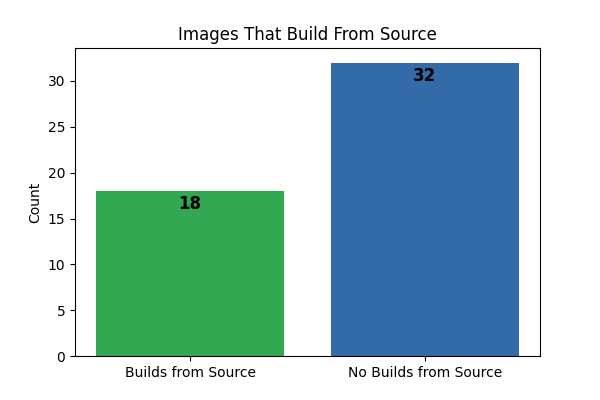
\includegraphics[width=0.4\textwidth]{Figs/libsec_tool/builds_plot.png}  
    \caption{Builds from Source vs No Builds}
    \label{fig:builds_plot}
    \end{figure}
  \end{frame}
\begin{frame}[fragile]
    \frametitle{Container Images that Build from Source (1)}
    \begin{minted}[fontsize=\small]{shell}
Images Built from Source:
 - library/memcached:1.6.32-bookworm
 - library/nginx:1.27.2-bookworm
 - library/redis:7.4.1-bookworm
 - library/postgres:17.1-bookworm
 - library/python:3.13.0-bookworm
 - library/node:23.2.0-bookworm
 - library/httpd:2.4.62-bookworm
 - library/golang:1.23.3-bookworm
 - library/ruby:3.3.6-bookworm
    \end{minted}
\end{frame}

\begin{frame}[fragile]
    \frametitle{Container Images that Build from Source (2)}
    \begin{minted}[fontsize=\small]{shell}
 - library/php:8.3.13-fpm-bookworm
 - nginxinc/nginx-unprivileged:1.27.2-bookworm
 - library/haproxy:3.0.6-bookworm
 - fluent/fluentd-kubernetes-daemonset:v1.17.1-debian-elasticsearch8-1.2
 - nodered/node-red:4.0.5-debian
 - library/perl:5.41.5-bookworm
 - library/buildpack-deps:bookworm
 - library/drupal:11.0.7-php8.3-fpm-bookworm
 - fluent/fluentd:v1.17.1-debian-1.1
    \end{minted}
\end{frame}

\begin{frame}[fragile]
    \frametitle{Container Images Not Built from Source (1)}
    \begin{minted}[fontsize=\small]{shell}
Images Not Built from Source:
 - bitnami/kubectl:1.31.2-debian-12-r6
 - library/mysql:8.0.40-bookworm
 - timberio/vector:0.42.0-debian
 - bitnami/postgresql:17.1.0-debian-12-r0
 - bitnami/redis:7.4.1-debian-12-r2
 - bitnami/sealed-secrets-controller:0.27.2-debian-12-r1
 - library/openjdk:24-jdk-bookworm
 - bitnami/mongodb:8.0.3-debian-12-r1
    \end{minted}
\end{frame}

\begin{frame}[fragile]
    \frametitle{Container Images Not Built from Source (2)}
    \begin{minted}[fontsize=\small]{shell}
 - library/debian:bookworm-20241111
 - bitnami/external-dns:0.15.0-debian-12-r5
 - kong/kong-gateway:3.8.1.0-20241114-debian
 - bitnami/mariadb:11.5.2-debian-12-r6
 - library/tomcat:11.0.0-jdk21-openjdk-bookworm
 - library/maven:3.9.9-amazoncorretto-23-debian
 - bitnami/rabbitmq:4.0.3-debian-12-r1
 - bitnami/nginx:1.27.2-debian-12-r3
 - itzg/minecraft-server:debian
    \end{minted}
\end{frame}


  % \begin{example}{E}
  %   an eample
  % \end{example}

  % \begin{alert}{A}
  %   an alert
  % \end{alert}




\section{Example Build Script inside Memcached}
\begin{frame}[fragile]
    \frametitle{Building Image: library/memcached:1.6.32-bookworm (1)}
    \begin{minted}[fontsize=\small]{shell}
RUN /bin/sh -c set -eux;
    apt-get update && apt-get install -y \
        ca-certificates gcc make wget perl;
    rm -rf /var/lib/apt/lists/*;

    wget -O memcached.tar.gz "$MEMCACHED_URL";
    echo "$MEMCACHED_SHA1  memcached.tar.gz" | sha1sum -c -;
    mkdir -p /usr/src/memcached;
    tar -xzf memcached.tar.gz -C /usr/src/memcached --strip-components=1;
    cd /usr/src/memcached;
    \end{minted}
\end{frame}

\begin{frame}[fragile]
    \frametitle{Building Image: library/memcached:1.6.32-bookworm (2)}
    \begin{minted}[fontsize=\small]{shell}
    gnuArch="$(dpkg-architecture --query DEB_BUILD_GNU_TYPE)";
    ./configure --build="$gnuArch" \
        --enable-extstore \
        --enable-sasl \
        --enable-sasl-pwdb \
        --enable-tls;
    
    nproc="$(nproc)";
    make -j "$nproc";
    make test PARALLEL="$nproc";
    make install;
    \end{minted}
\end{frame}


\section{Dlopen - Dlsym analysis}
\begin{frame}[fragile]
  \frametitle{Dlopen Dlsym analysis}
  Reminder:
  \small
    \begin{minted}[breaklines]{python}
       pkg_analyze.py:785 output_stats() 
        In total, Packages of this container had 942 CVEs         pkg_analyze.py:785
        In that, Packages, that have libraries, that have symbols have 840 CVEs                                                
        In that, Packages, that have functions related to cves, have 177 related CVEs                                          
        In that, Packages, that have their vuln functions called, have 85 related CVEs.  
    \end{minted}
    \normal
%   %  Syspart Added:
  %   \begin{minted}[breaklines,breakanywhere]{c++}  
  %     int signedOrZero; // private member variable 
  %     ...
  %     setSignedOrZero(); 
  %     ... 
  %     getSignedOrZero();
  %     // My Guess
  %   \end{minted}
  %   \vspace{20pt}
\end{frame}

\begin{frame}[fragile]
  % \frametitle{\texttt{src/analysis/jumptableDetection.$*$}}
  %  Syspart Added:
  %   \begin{minted}[breaklines,breakanywhere]{c++}  
  %     auto jsAssembly = js->getInstruction()
  %     ->getSemantic()->getAssembly();
  %     if(jsAssembly->getId() == X86_INS_MOVZX)
  %         info->signedOrZero=0;
  %     else if ((jsAssembly->getId() == X86_INS_MOVSB)  || ...
  %     || (jsAssembly->getId() == X86_INS_MOVSXD))
  %     {
  %         info->signedOrZero=1;
  %     }
  %     // this check is added wherever info is edited.
  %     // info is of type JumptableInfo.
  %     // later signedOrZero is also used in src/pass/jumptablepass.cpp
  %   \end{minted}
  %   \vspace{20pt}
\end{frame}

% \section{Egalito \texttt{usedef} changes}
\begin{frame}[fragile]
%   \frametitle{\texttt{src/analysis/usedef.h}}
%   the following is added in class Usedef. I couldn't understand purpose of this class.
%   \begin{minted}[breaklines]{c++}
%     void fillLea(UDState *state, AssemblyPtr assembly);
%     // added below
%     void fillCMov(UDState *state, AssemblyPtr assembly);
%     // added below
%     void fillX86Ret(UDState *state, AssemblyPtr assembly);
%     void fillMovabs(UDState *state, AssemblyPtr assembly);
%     ...
%     // added below
%     long int getOffset() { return offset; }
% \end{minted}
%     \vspace{20pt}
\end{frame}
\begin{frame}[fragile]
  % \frametitle{\texttt{src/analysis/usedef.cpp}}
  %  Syspart Added:
  %   \begin{minted}[breaklines,breakanywhere]{c++}  
  %     void DefList::set(int reg, TreeNode *tree) {
  %         {X86_INS_CMOVA,     &UseDef::fillCMov },
  %         {X86_INS_CMOVAE,    &UseDef::fillCMov },
  %         {X86_INS_CMOVB,     &UseDef::fillCMov },
  %         {X86_INS_CMOVBE,    &UseDef::fillCMov },
  %         {X86_INS_CMOVE,     &UseDef::fillCMov },
  %     ... // some other fillcmov
  %         {X86_INS_RET,       &UseDef::fillX86Ret},
  %           }
  %   // I couldn't understand purpose of deflist exactly.
    
  %   \end{minted}
  %   \vspace{20pt}
\end{frame}


\begin{frame}[fragile]
%   \frametitle{\texttt{src/analysis/usedef.cpp}}
%   \begin{minted}[breaklines]{c++}
%      void UseDef::fillRegToReg(UDState *state, AssemblyPtr assembly) {
% ...
%     else if( id == X86_INS_CMOVA
%         || id == X86_INS_CMOVAE
%         || id == X86_INS_CMOVB
%         || id == X86_INS_CMOVBE
%         || id == X86_INS_CMOVE
%           // some other cmov s
%         || id == X86_INS_CMOVS)
%     {
%         tree = TreeFactory::instance().make<TreeNodePhysicalRegister>(
%             reg0, width0);
%         state->addRegDef(reg1, tree);
%         working->addToRegSet(reg1, state);
%         return;
%     }

%     \end{minted}
%     \vspace{20pt}
\end{frame}



